\documentclass[12pt,a4paper]{article}

% ── Packages ──────────────────────────────────────────────────────────────────
\usepackage[margin=1in]{geometry}
\usepackage{amsmath,amssymb}
\usepackage{graphicx}
\usepackage{booktabs}
\usepackage{enumitem}
\usepackage{hyperref}
\usepackage{xcolor}
\usepackage{tikz}
\usetikzlibrary{arrows.meta,positioning,shapes.geometric,fit,backgrounds,calc}
\usepackage{titlesec}
\usepackage{fancyhdr}
\usepackage[T1]{fontenc}
\usepackage{lmodern}

% ── Page style ────────────────────────────────────────────────────────────────
\pagestyle{fancy}
\fancyhf{}
\fancyhead[L]{\small IDCR --- Project Proposal}
\fancyhead[R]{\small \thepage}
\renewcommand{\headrulewidth}{0.4pt}

\hypersetup{
  colorlinks=true,
  linkcolor=blue!60!black,
  citecolor=blue!60!black,
  urlcolor=blue!60!black
}

\titleformat{\section}{\large\bfseries}{}{0em}{}[\vspace{-0.5em}\rule{\textwidth}{0.4pt}]
\titleformat{\subsection}{\normalsize\bfseries}{}{0em}{}

% ── Title ─────────────────────────────────────────────────────────────────────
\title{%
  \vspace{-1.5cm}
  {\LARGE\bfseries Information-Directed Conformal Retrieval}\\[6pt]
  {\large A Decision-Theoretic Framework for Autonomous\\
   Uncertainty-Aware Financial Recommendations}\\[10pt]
  {\normalsize\textsc{Project Proposal}}
}

\date{\today}

% ══════════════════════════════════════════════════════════════════════════════
\begin{document}
\maketitle
\thispagestyle{fancy}

% ──────────────────────────────────────────────────────────────────────────────
\section{Problem and Motivation}
% ──────────────────────────────────────────────────────────────────────────────

Current AI systems for financial recommendations suffer from a fundamental limitation: they produce confident-sounding outputs with no calibrated measure of uncertainty.
A system that recommends ``allocate 40\% to technology stocks'' without quantifying \emph{how uncertain} that recommendation is can be actively dangerous in high-stakes domains.

Retrieval-Augmented Generation (RAG) partially addresses this by grounding recommendations in retrieved documents (analyst reports, SEC filings, market data).
However, existing RAG pipelines treat retrieval as a disconnected preprocessing step---documents are selected based on semantic similarity, not on whether they actually \emph{reduce decision uncertainty}.

We propose \textbf{Information-Directed Conformal Retrieval (IDCR)}, a framework that:
\begin{enumerate}[nosep]
  \item Selects documents \emph{because} they reduce uncertainty in the downstream recommendation.
  \item Provides \textbf{distribution-free coverage guarantees}---prediction sets that provably contain the optimal recommendation with a user-specified probability (e.g., 90\%).
  \item Formalizes the entire pipeline as end-to-end autonomous decision making, mirroring how a human financial advisor operates.
\end{enumerate}

% ──────────────────────────────────────────────────────────────────────────────
\section{The Human Decision-Making Analogy}
% ──────────────────────────────────────────────────────────────────────────────

Our framework is motivated by how expert human advisors make decisions.
We formalize each stage with principled techniques:

\begin{center}
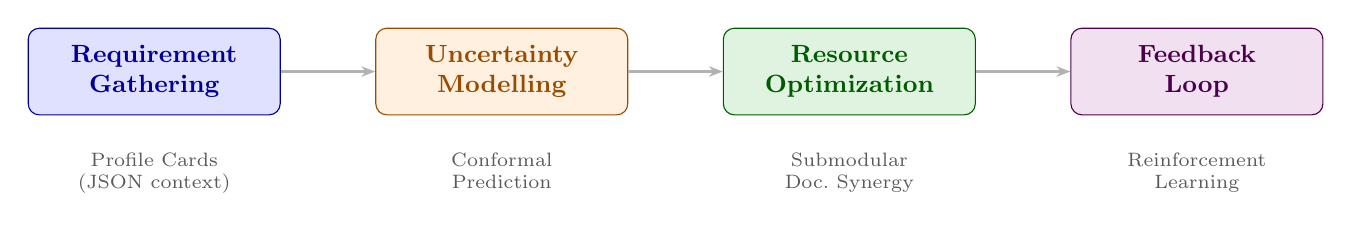
\begin{tikzpicture}[
  node distance=0.4cm and 1.2cm,
  stage/.style={draw, rounded corners=4pt, minimum width=3.2cm,
                minimum height=1.1cm, align=center, font=\small\bfseries,
                fill=#1!12, draw=#1!60!black, text=#1!60!black},
  tech/.style={font=\scriptsize, align=center, text=gray!70!black},
  arr/.style={-{Stealth[length=5pt]}, thick, gray!60}
]
  \node[stage=blue]                     (req)  {Requirement\\Gathering};
  \node[stage=orange, right=of req]     (unc)  {Uncertainty\\Modelling};
  \node[stage=green!60!black, right=of unc]  (opt)  {Resource\\Optimization};
  \node[stage=violet, right=of opt]     (fb)   {Feedback\\Loop};

  \node[tech, below=0.35cm of req]  {Profile Cards\\(JSON context)};
  \node[tech, below=0.35cm of unc]  {Conformal\\Prediction};
  \node[tech, below=0.35cm of opt]  {Submodular\\Doc.\ Synergy};
  \node[tech, below=0.35cm of fb]   {Reinforcement\\Learning};

  \draw[arr] (req) -- (unc);
  \draw[arr] (unc) -- (opt);
  \draw[arr] (opt) -- (fb);
\end{tikzpicture}
\end{center}

\vspace{-0.5em}

\begin{enumerate}[leftmargin=*,nosep]
  \item \textbf{Requirement Gathering $\to$ Profile Cards.}
    A financial advisor begins by understanding the client.
    We encode user context as structured \emph{profile cards}---JSON objects capturing risk tolerance, investment horizon, sector preferences, current holdings, constraints, and demographic information.
    These serve as the complete context for all downstream reasoning.

  \item \textbf{Uncertainty Modelling $\to$ Conformal Prediction.}
    An advisor mentally gauges how confident they are.
    We use \emph{conformal prediction} to construct prediction sets (``the optimal allocation lies in this region with 90\% confidence'') that come with distribution-free, finite-sample guarantees---no assumptions about the data-generating process.

  \item \textbf{Maximum Resource Utilization $\to$ Submodular Retrieval \& Document Synergy.}
    An advisor selects the most complementary research sources.
    We prove that uncertainty reduction is \emph{submodular} (diminishing returns), enabling efficient greedy document selection.
    We further characterize when documents are \emph{synergistic}---combinations that together reveal information unavailable from any individual document.

  \item \textbf{Feedback Loop $\to$ Reinforcement Learning (IDS).}
    An advisor refines their process over time.
    We use Information-Directed Sampling to balance exploration (learning which documents help) with exploitation (using known-good documents), with provable regret bounds.
\end{enumerate}

% ──────────────────────────────────────────────────────────────────────────────
\section{Task: Portfolio Allocation Under Uncertainty}
% ──────────────────────────────────────────────────────────────────────────────

\subsection{Why Portfolio Allocation?}
We instantiate IDCR on \textbf{portfolio weight recommendation}, where:
\begin{itemize}[nosep]
  \item The user provides a profile card (risk tolerance, horizon, constraints).
  \item The document corpus contains analyst reports, earnings summaries, macro indicators, and news.
  \item The system outputs a portfolio weight vector $w \in \mathbb{R}^d$ over $d$ asset classes.
  \item The ground truth is the ex-post optimal allocation (computable since we control the data-generating process).
\end{itemize}

This task is ideal because: the conformal prediction set is a geometric ellipsoid in weight space with directly interpretable meaning; documents have natural precision semantics (a tech analyst report narrows uncertainty along the technology dimension); and document synergy arises naturally (a macro report combined with a sector report reveals regime-specific information neither provides alone).

\subsection{Profile Card Schema}
Each user is encoded as a structured JSON profile card:

\begin{center}
\small
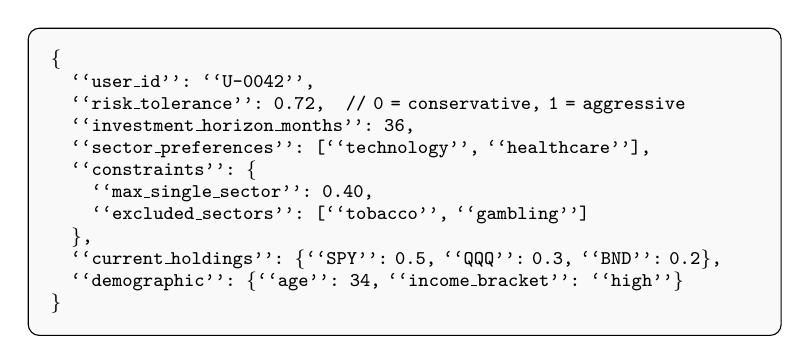
\begin{tikzpicture}[
  every node/.style={font=\ttfamily\scriptsize}
]
\node[draw, rounded corners, fill=gray!5, text width=9cm, inner sep=8pt, align=left] {
\{\\
\quad ``user\_id'': ``U-0042'',\\
\quad ``risk\_tolerance'': 0.72,\quad // 0 = conservative, 1 = aggressive\\
\quad ``investment\_horizon\_months'': 36,\\
\quad ``sector\_preferences'': [``technology'', ``healthcare''],\\
\quad ``constraints'': \{\\
\qquad ``max\_single\_sector'': 0.40,\\
\qquad ``excluded\_sectors'': [``tobacco'', ``gambling'']\\
\quad \},\\
\quad ``current\_holdings'': \{``SPY'': 0.5, ``QQQ'': 0.3, ``BND'': 0.2\},\\
\quad ``demographic'': \{``age'': 34, ``income\_bracket'': ``high''\}\\
\}
};
\end{tikzpicture}
\end{center}

% ──────────────────────────────────────────────────────────────────────────────
\section{Proposed Methodology (Overview)}
% ──────────────────────────────────────────────────────────────────────────────

The IDCR pipeline operates in three phases:

\textbf{Phase 1: Sequential Document Retrieval.}
Given a user profile card and a corpus of financial documents, the system iteratively selects $k$ documents.
At each step, it scores every candidate document by how much it would reduce the uncertainty ellipsoid volume, augmented by an exploration bonus that accounts for uncertainty in the document's informativeness itself.
The key theoretical result is that this selection objective exhibits \emph{diminishing returns} (submodularity), so a simple greedy algorithm achieves at least 63\% of the optimal uncertainty reduction.

\textbf{Phase 2: Conformal Calibration.}
Using a held-out calibration dataset, the system computes a threshold such that the resulting prediction ellipsoid provably contains the true optimal allocation with probability $\geq 1-\alpha$.
This guarantee is \emph{distribution-free}---it holds regardless of the true data distribution, requiring only that calibration and test data are exchangeable.

\textbf{Phase 3: Recommendation with Uncertainty Decomposition.}
The system outputs: (a) a point estimate $\hat{w}$ (the recommended portfolio weights), (b) a prediction set $C_\alpha$ with coverage guarantees, and (c) an uncertainty decomposition showing how much uncertainty comes from the user profile ambiguity, from document relevance uncertainty, and from irreducible market noise.

% ──────────────────────────────────────────────────────────────────────────────
\section{Evaluation Strategy}
% ──────────────────────────────────────────────────────────────────────────────

\subsection{Baselines}
We compare IDCR against four baselines representing increasing levels of sophistication:

\begin{center}
\small
\renewcommand{\arraystretch}{1.3}
\begin{tabular}{@{}lp{8cm}@{}}
\toprule
\textbf{System} & \textbf{Description} \\
\midrule
Zero-Shot (no tools) & LLM receives only the user profile card; produces allocation directly. \\
Zero-Shot (with tools) & LLM receives profile card + access to web search and calculator tools. \\
Few-Shot ($\pm$ tools) & LLM receives 3--5 example (profile $\to$ allocation) demonstrations. \\
Standard RAG & Cosine-similarity retrieval of top-$k$ documents + LLM generation. \\
\textbf{IDCR (Ours)} & Submodular retrieval $\to$ conformal calibration $\to$ allocation with uncertainty. \\
\bottomrule
\end{tabular}
\end{center}

\subsection{Metrics}
\begin{center}
\small
\renewcommand{\arraystretch}{1.3}
\begin{tabular}{@{}llp{6.5cm}@{}}
\toprule
\textbf{Metric} & \textbf{Type} & \textbf{What It Measures} \\
\midrule
MSE / Cosine Similarity & Decision quality & How close $\hat{w}$ is to the true optimal $w^*$. \\
Empirical Coverage & Calibration & Does the 90\% set contain $w^*$ $\geq$90\% of the time? \\
Set Volume & Efficiency & How tight is the prediction region. \\
Sharpe Ratio & Financial & Risk-adjusted return of the recommended portfolio. \\
Max Drawdown & Financial & Worst-case loss---measures tail risk. \\
Robustness & Stress test & Performance under regime shift (calibration vs.\ test distribution mismatch). \\
\bottomrule
\end{tabular}
\end{center}

\subsection{Key Hypothesis}
\emph{IDCR will match or exceed baselines on point-estimate accuracy (MSE, Sharpe) while being the \textbf{only} system that provides calibrated uncertainty quantification (valid coverage, tight set volume).}
The baselines produce point estimates with no principled uncertainty---even when they happen to be accurate, they cannot distinguish ``I'm confident'' from ``I'm guessing.''

% ──────────────────────────────────────────────────────────────────────────────
\section{Experiments}
% ──────────────────────────────────────────────────────────────────────────────

\begin{enumerate}[nosep, leftmargin=*]
  \item \textbf{Submodularity Verification}: Empirically verify diminishing returns by plotting marginal uncertainty reduction as the retrieved set grows.
  \item \textbf{Greedy Approximation Quality}: Compare greedy retrieval to brute-force optimal for small $k$ to validate the $\geq$63\% guarantee.
  \item \textbf{RL vs.\ Greedy Under Synergy}: Train RL policy on corpora with controlled synergy structure; verify RL outperforms greedy only when synergistic documents exist.
  \item \textbf{Coverage Verification}: Confirm distribution-free coverage across all retrieval policies (random, greedy, RL) at multiple $\alpha$ levels.
  \item \textbf{Baseline Comparison}: Full comparison of all 5 systems on the portfolio allocation task across all metrics.
  \item \textbf{Efficiency--Coverage Pareto}: Plot the frontier of (coverage rate, set volume) for varying $\alpha$ and retrieval budget $k$.
\end{enumerate}

% ──────────────────────────────────────────────────────────────────────────────

% ──────────────────────────────────────────────────────────────────────────────
\section{Expected Contributions}
% ──────────────────────────────────────────────────────────────────────────────

\begin{enumerate}[nosep]
  \item \textbf{Formalization}: First framework connecting document retrieval to conformal set minimization for autonomous decision making.
  \item \textbf{Theory}: Submodularity proof enabling efficient retrieval with approximation guarantees; interaction tensor characterizing when RL is needed.
  \item \textbf{System}: End-to-end pipeline from profile cards through uncertainty-aware document retrieval to calibrated portfolio recommendations.
  \item \textbf{Evaluation}: Comprehensive comparison showing that principled retrieval yields both better decisions and the only formally valid uncertainty estimates.
\end{enumerate}

\end{document}